\documentclass[main.tex]{subfiles}

\begin{document}
\chapter{Many-body physics\label{chap:many-body-physics}}
%\epigraph{It's a secret to everybody.}{a Moblin in \textit{The Legend of Zelda}}

%\section{The electronic structure problem\label{sec:theory_schrödinger}}

In solid state physics, the Hamiltonian describing the interacting nuclei and electrons in the solid is well known, as all interactions except Coulomb interaction can safely be ignored at the mass and energy scales at which the electrons and nuclei reside.
This still very general problem consisting of both the electronic and nuclei degrees of freedom can be simplified in a first step by employing the Born-Oppenheimer approximation.
The approximation assumes the nuclei to be fixed point charges which create a potential for the \(N\) interacting electrons, so that the electronic part can be solved independently using the nuclei positions \(\vb{R}_{\alpha}\) as a parameter.

The problem is then described by the time-independent Schrödinger equation
\begin{equation}\label{}
    \ope{H} \Psi (\vb{r}_1, \ldots, \vb{r}_N) = E \Psi (\vb{r}_1, \ldots, \vb{r}_N)
\end{equation}
with the Hamiltonian in first quantization (\(i\) running over the electrons, \(\alpha, \beta\) over the nuclei)
\begin{align}
    \ope{H} &= \ope{T}_e + \ope{U}_{e-e} + \ope{V}_{n-e} + \ope{W}_{n-n} \\
    &= -\sum_i \frac{1}{2} \nabla^2_i 
    + \frac{1}{2} \sum_{i \neq j} \frac{1}{\vert \vb{r}_i - \vb{r}_j \vert} 
    - \sum_i \sum_{\alpha} \frac{Z_{\alpha}}{\vert \vb{r}_i 
    - \vb{R}_{\alpha} \vert} 
    + \frac{1}{2} \sum_{\alpha \beta} \frac{Z_{\alpha} Z_{\beta}}{R_{\alpha \beta}} 
\end{align}
where:
\begin{itemize}
    \item \(\ope{T}_e\) is the kinetic energy of the electrons
    \item \(\ope{U}_{e-e}\) is the Coulomb interaction between the electrons and
    \item \(\ope{V}_{n-e}\) is the potential energy of the electrons in the field of the nuclei
    \item \(\ope{W}_{n-n}\) is the Coulomb interaction between the nuclei
\end{itemize}
The terms \(\ope{V}_{n-e}\) and \(\ope{W}_{n-n}\) can then be combined into an external potential \(V\) for the interacting electrons, so that the Hamiltonian reads
\begin{equation}\label{eq:solid_state_hamiltonian}
    \ope{H} = \ope{T} + \ope{U} + \ope{V}
\end{equation}
This Hamiltonian will be used in the further development of the underlying theory for this thesis.

\section{Density Functional Theory\label{sec:theory_dft}}

A direct solution to the electronic structure problem, this meaning obtaining the ground-state many-body wave function \(\Psi (\vb{r_1}, \ldots, \vb{r}_N)\) for a given potential is analytically impossible even for a small number of electrons compared to the number of electrons in a macroscopic crystal.
As such, the need for good approximations to obtain results for real world
systems is high.
One particularly successful approach is \acrfull{dft}.
In the following section, the theoretical framework of \acrshort{dft} will be reviewed, the outline of which can be found in any literature on solid state physics \cite{marzari_ab-initio_1996}.

\subsection{Hohenberg-Kohn theorems}

The start for DFT is the exact reformulation of the outlined electronic structure problem by Hohenberg and Kohn \cite{hohenberg_inhomogeneous_1964}.
This reformulation uses the ground state density of the electronic system \(n_0 (r)\) as the basic variable.
To achieve this, Hohenberg and Kohn \cite{hohenberg_inhomogeneous_1964} formulated two theorems, which demonstrate that the ground state properties of an electronic system can be described using the ground state density (the proof of those theorems is omitted here, but can be found in the original paper \cite{hohenberg_inhomogeneous_1964} or any publication on \acrshort{dft} \cite{marzari_ab-initio_1996}):
\begin{enumerate}[I]
    \item The external potential is a unique functional of the ground state density.
    \item The ground state energy minimizes the energy functional,
    \[E[n(\vb{r})] > E_0 \;\forall\; n(\vb{r}) \neq n_0 (\vb{r})\,.\]
\end{enumerate}
These theorems proof the existence and uniqueness of the energy functional \(E[n(\vb{r})]\), but a concrete expression for it cannot be given.
As the ground state wave function is a functional of the ground state density, a formal definition of the energy functional can be written as
\begin{align*}
    E[n(\vb{r})] &= \expval{\ope{H}}{\Psi} \\
    &= \expval{\ope{T} + \ope{U} + \ope{V}}{\Psi} \\
    &= \expval{\ope{T} + \ope{U}}{\Psi} + \int \dd{\vb{r}^{\prime}} \Psi^* (\vb{r}^{\prime}) V(\vb{r}^{\prime}) \Psi (\vb{r}^{\prime})\,.
\end{align*}
Defining the universal functional \(F[n(\vb{r})] = \expval{T + U}{\Psi}\), which is material independent and writing \(n (\vb{r}^{\prime}) = \Psi^* (\vb{r}^{\prime}) \Psi (\vb{r}^{\prime})\), the energy functional becomes
\begin{equation}\label{eq:hohenberg_kohn_energy_functional}
    E[n(\vb{r})] = F[n(\vb{r})] + \int \dd{\vb{r}^{\prime}} V(\vb{r}^{\prime}) n (\vb{r}^{\prime})\,.
\end{equation}
This is just a formal definition, as all the formerly mentioned complication of the Hamiltonian \ref{eq:solid_state_hamiltonian} now lie in the functional \(F[n(\vb{r})]\).
With a known or well approximated universal functional \(F[n(\vb{r})]\), the Hohenberg-Kohn theorems provide a great simplification for finding the ground state properties of a solid state system, as the problem is now only a variational problem with 3 spatial coordinates instead of \(3N\) coordinates when trying to solve the full Hamiltonian.


\subsection{Kohn-Sham equations}

Kohn and Sham proposed an approach to handling interacting many-body systems by introducing an auxiliary non-interacting system of electrons \cite{kohn_self-consistent_1965}
\begin{equation}\label{eq:kohn_sham_hamiltonian}
    H_0 = \sum_i^{N_e} \frac{p_i^2}{2m} + v_{KS} (\vb{r}_i)\,.
\end{equation}
With a correction potential \(v_{KS}\) such that the ground state charge density for the auxiliary and the interacting system are the same.
This introduces a new set of orthonormal wave functions, the solutions to the non-interacting problem \(\Psi_i\).
The density for this system is calculated as
\begin{equation}\label{eq:density_ks_states}
    n(\vb{r}) = \sum_{i=1}^N \vert \Psi_i (\vb{r}) \vert^2\,.
\end{equation}
The restriction of equality of the ground state densities for the interacting and the non-interacting system makes it possible to calculate all properties of the interacting system just by solving the non-interacting system (using the Hohenberg-Kohn theorems).
This connection is shown in fig. \ref{fig:kohn_sham_dft_schema}.
\begin{figure}[ht!]
    \centering
    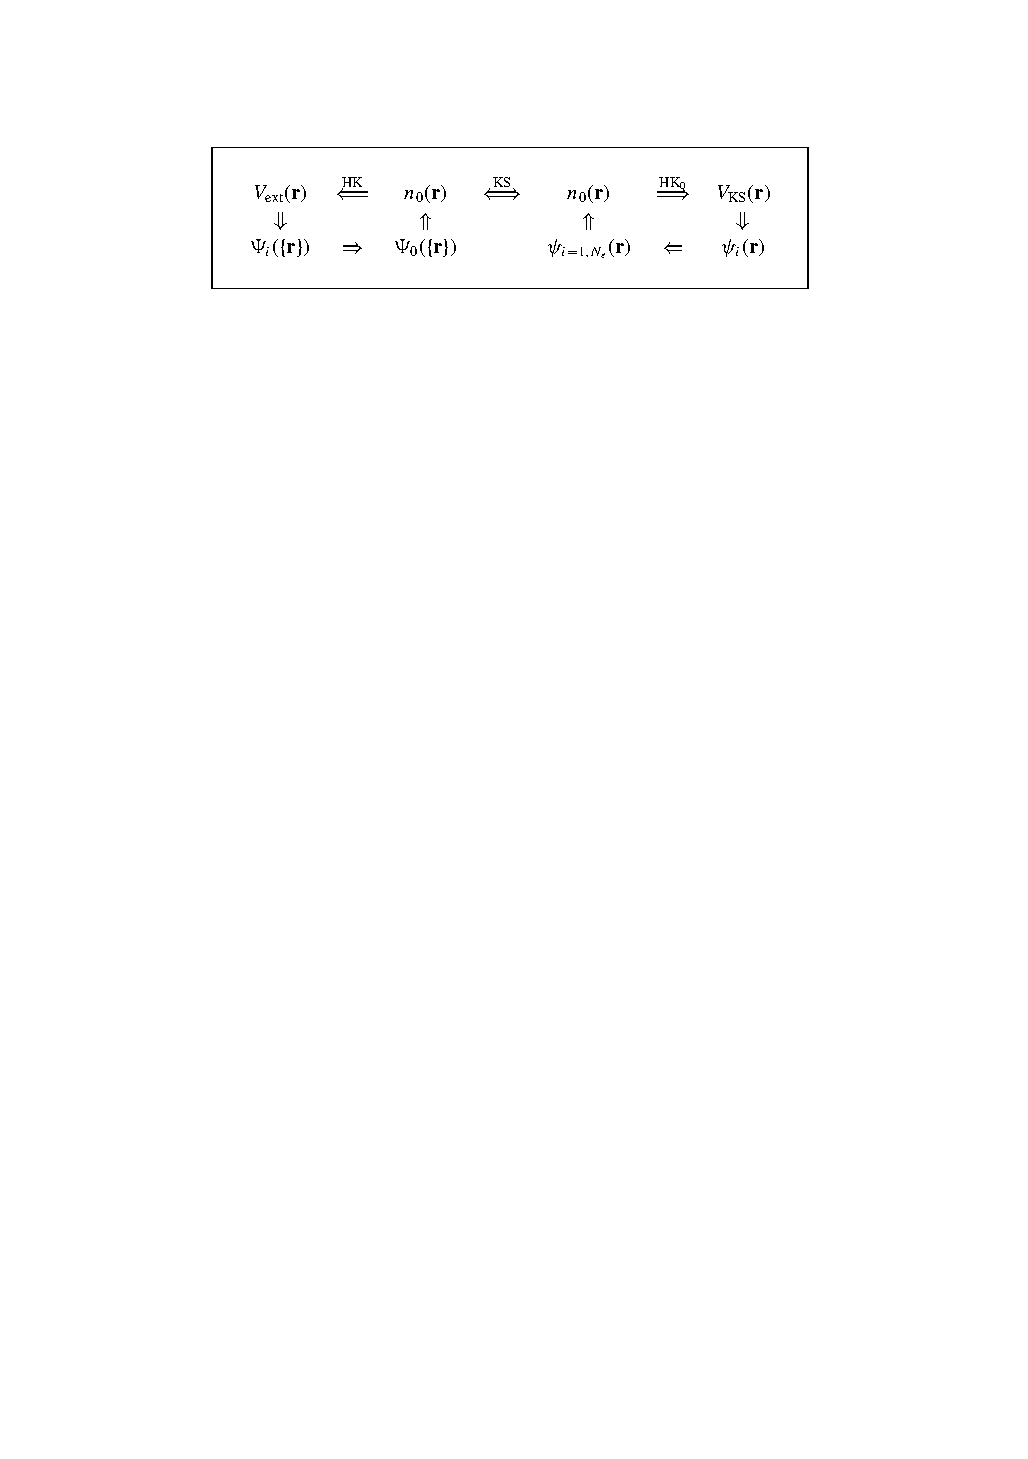
\includegraphics[width=0.7\textwidth]{martins_ks_dft_schema.pdf}
    \caption{CAPTION \cite[137]{martin_electronic_2004}}
    \label{fig:kohn_sham_dft_schema}
\end{figure}

The kinetic energy of such a non-interacting problem can be easily calculated as sum over all electrons
\begin{equation}
    T_S [n(\vb{r})] = - \frac{1}{2} \sum_{i=1}^{N_e} \int \dd[3]{r} \Psi_i^* (\vb{r}) \Delta \Psi_i (\vb{r})\,.
\end{equation}
With the help of this system and the classical electrostatic energy 
\begin{equation}
    E_H [n(\vb{r})] = \frac{1}{2} \int \int \dd[3]{r_1} \dd[3]{r_2} \frac{n(\vb{r}_1) n(\vb{r}_2)}{\vert \vb{r}_1 - \vb{r}_2 \vert}
\end{equation}
an ansatz for the total energy functional in eq. \ref{eq:hohenberg_kohn_energy_functional} can be written as
\begin{equation}
    E[n(\vb{r})] = T_S [n(\vb{r})] + E_H [n(\vb{r})] + E_{XC} [n(\vb{r})] + \int \dd{\vb{r}^{\prime}} V(\vb{r}^{\prime}) n (\vb{r}^{\prime})\,.
\end{equation}
where now \(E_{XC} [n(\vb{r})]\) is a functional of the density accounting for all exchange and correlation effects not present in the non-interacting electron system.
The success of \acrshort{dft} lies in the fact that \(E_{XC}\) contributes only a small part of the total energy and can be approximated in a useful manner. \todo{source, more explanation}

Using that form of \(E[n(\vb{r})]\), from the variational problem (with a Lagrange parameter introduced to ensure the orthonormality of the states \(\Psi_i\))
\begin{align}
     \delta \left( E [n(\vb{r})] - \sum_j \lambda_j \left[\int \dd[3]{r} \vert \Psi_j \vert^2 - 1 \right] \right) = 0
\end{align}
a set of single particle, Schrödinger-like equations can be derived:
\begin{equation}\label{eq:kohn-sham-equations}
    \left(-\frac{1}{2} \Delta + \frac{1}{2} \int \dd[3]{r^{\prime}} \frac{n(\vb{r}^{\prime})}{\vert \vb{r} - \vb{r}^{\prime} \vert} + \fdv{E_{XC}}{n(\vb{r})} + V\right) \Psi_i (\vb{r}) = \lambda_i \Psi_i (\vb{r})\,.
\end{equation}
Schrödinger-like in this context means, that with the identification of the Hartree potential \(V_H = \frac{1}{2} \int \dd[3]{r^{\prime}} \frac{n(\vb{r}^{\prime})}{\vert \vb{r} - \vb{r}^{\prime} \vert}\) and the exchange-correlation potential \(V_{XC} = \fdv{E_{XC}}{n(\vb{r})}\) the potential \(v_{KS}\) in eq. \ref{eq:kohn_sham_hamiltonian} is
\begin{equation}
    v_{KS} =  V_H + V_{XC} + V = \frac{1}{2} \int \dd[3]{r^{\prime}} \frac{n(\vb{r}^{\prime})}{\vert \vb{r} - \vb{r}^{\prime} \vert} + \fdv{E_{XC}}{n(\vb{r})} + V\,.
\end{equation}
Eq. \ref{eq:kohn-sham-equations} become the \acrshort{kohn_sham} equations
\begin{equation}
    \left(- \frac{1}{2} \Delta + v_{KS}\right) \Psi_i (\vb{r}) = \epsilon_i \Psi_i (\vb{r})\,.
\end{equation}
Importantly, the potential \(v_{KS}\) depends on the solutions \(\Psi_i (\vb{r})\), as \(V_H\) and \(V_{XC}\) include the density \(n(\vb{r})\).
The problem thus is a self-consistency problem, meaning the density used for calculating the potentials and the obtained solution only agree for the exact solution.
Arriving at a solution consists then of iterating the process of obtaining a new set of potentials from the solution and solving the \acrshort{kohn_sham} equations again.

\subsection{Pseudopotentials and basis set}\label{sub:theory_basis_set}

In order to represent the states and operators in eq. \ref{eq:kohn-sham-equations}, a basis set has to be chosen.
Bloch's theorem states that the in case of a periodic external potential, which makes the Hamiltonian commute with translation operators for translation by a lattice vector, the common eigenstates of these operators are:
\begin{equation}
    \Psi (\vb{r}) = \Psi_{n \vb{k}} (\vb{r}) = e^{i \vb{k} \cdot \vb{r}} u_{n \vb{k}} (\vb{r})
\end{equation}
where \(\vb{k}\) is the quasi-momentum and \(u_{n \vb{k}} (\vb{r})\) has the periodicity of the unit cell.
A natural choice to represent \(u_{n \vb{k}} (\vb{r})\) is the discrete set of plane waves \(\ket{\vb{G}}\)
\begin{align}
    \bra{\vb{r}} \ket{\vb{G}} &= \frac{1}{\sqrt{V}} e^{i \vb{G} \vb{r}} \\
    \implies \Psi_{n \vb{k}} (\vb{r}) &= \sum_{\vb{G}} c_{n \vb{k}, \vb{G}} e^{i (\vb{k} + \vb{G}) \vb{r}}
\end{align}
where \(\vb{G}\) is a reciprocal lattice vector. \todo{right like that? do the plane waves have the periodicity of the unit cell?}
With that choice of basis set, the kinetic energy is easily calculated:
\begin{equation}
    \bra{\Psi_{n \vb{k}} (\vb{r})} - \nabla^2 \ket{\Psi_{n \vb{k}} (\vb{r})} = \sum_{\vb{G}} c_{n \vb{k}, \vb{G}}^2 \vert \vb{k} + \vb{G} \vert^2
\end{equation}
Another important consequence of this choice of basis set is that the electron density (eq. \ref{eq:density_ks_states}) now becomes an integral over the Brillouin zone, which for numerical computation has to be approximated by a sum over a finite set of k points. \todo{concrete formula for that?}

One problem of this choice of basis set lies in the fact that the lower energy core electrons are very localized around the cores and as such need a lot of basis functions.
Because the higher orbitals have to be orthogonal to the lower orbitals, they must also have features on the length scale of the core electrons, which means more basis functions are needed to describe them accurately.

Importantly, the core electrons don't contribute much to the electronic structure problem, so an approach to make the calculations more economically is to introduce an effective screened potential which describes the nuclear potential as well as the states close to the nucleus.
These potentials are called \acrfull{pp} and the orbitals constructed with them are smooth functions and can be accurately represented with a small number of basis functions.
This fact can be used in computation by introducing a \emph{cutoff energy} \(E_{cutoff}\) which limits the number of basis functions by using only expansion coefficents with \(\vert \vb{k} + \vb{G} \vert \leq E_{cutoff}\) \todo{should be (k+G) to the power of 2 right? also maybe concrete formula for that}. Besides the number of k points, this is the second variable which can influences the computation time of \acrshort{dft} calculations.

With Fast Fourier Transforms \gls{fft}, an efficient algorithm exists to transform from (discrete) real to (discrete) reciprocal space so every expectation value can be calculated in the optimal representation: in reciprocal space for the kinetic energy and in real space for the pseudopotentials.

\todo{talk about scf loop here!}

\begin{wrapfigure}{l}{0.5\textwidth}
\centering
\begin{tikzpicture}[
    squarednode/.style={rectangle, draw=purple!60, fill=purple!5, thick, minimum size=5mm, text centered, text width=3cm,},
    node distance=0.5cm]
    %Nodes
    \node[squarednode]      (init)          {initial \(n(\vb{r})\)};
    \node[squarednode]      (step_1)    [below= of init]  {calculate \(v_H [n(\vb{r})]\) and \(v_{XC} [n(\vb{r})]\)};
    \node[squarednode]      (step_2)    [below= of step_1]      {fourier transform potentials};
    \node[squarednode]      (step_3)    [below= of step_2]      {solve \acrshort{kohn_sham} equations in reciprocal space};
    \node[squarednode]      (step_4)    [below= of step_3]      {fourier transform wavefunctions};
    \node[squarednode]      (step_5)    [below= of step_4]      {calculate \(n(\vb{r})\) and \(E [n(\vb{r})]\)};
    \node[squarednode]      (done)      [below= of step_5]      {done if change in \(E\) is small enough};
    
    %Lines
    \draw[->] (init.south) -- (step_1.north);
    \draw[->] (step_1.south) -- (step_2.north);
    \draw[->] (step_2.south) -- (step_3.north);
    \draw[->] (step_3.south) -- (step_4.north);
    \draw[->] (step_4.south) -- (step_5.north);
    \draw[->] (step_5.east) to [out=30,in=-30] (step_1.east);
    \draw[->] (step_5.south) -- (done.north);
\end{tikzpicture}
\label{fig:diagram_scf_calculations}
\caption{Flowchart of an algorithm to solve the \acrshort{kohn_sham} equations}
\end{wrapfigure}

tt

\section{Density Functional Perturbation Theory}\label{sec:theory_dfpt}

\todo{dfpt!!!}

\section{Examined systems}

\subsection{Silicon}

\subsection{\TaS}


\end{document}
